% solution_2_pulses.tex
% by Troy Hix, March 2005
%----------------------------------------------------------------------------
\begin{figure}
\centering
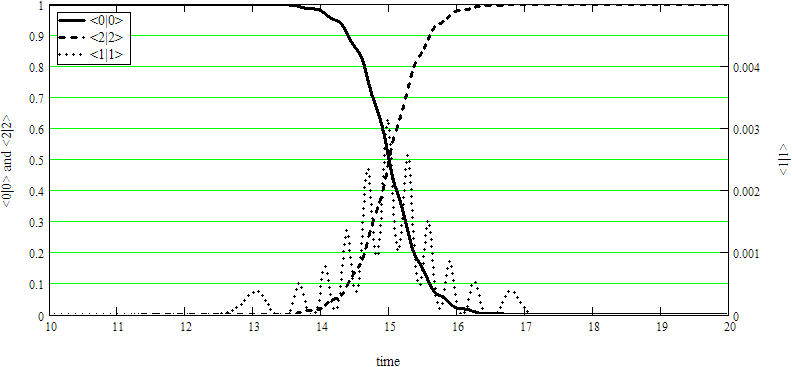
\includegraphics[width=5.00in]
{solution_2-stronger_energy_levels/solution_2-stronger_energy_levels.png}\\
\caption[Two color optimal solution - increased pulse amplitude]{Two color optimal solution - increased pulse amplitude. $\braket{\Psi}{\Psi}$'s behavior at an optimum with increased pulse amplitudes. Note that $\braket{0}{0}$ and $\braket{2}{2}$ are shown at a different scale than $\braket{1}{1}$. Notice the decrease in the average height of $\braket{1}{1}$ when compared to $\braket{1}{1}$ in figure \ref{solution 2 energy levels}. For this solution $\Delta_{\alpha}=-1.3146820926$ and $A=19.5606505329$ (26.511 times the area of the $\pi$--pulse).}
\label{solution 2-stronger energy levels}
\end{figure} 
%----------------------------------------------------------------------------
